\documentclass[12pt]{article}

\usepackage[justification=centering]{caption}
\usepackage[pdftex]{graphicx}
\usepackage{amsmath}
\usepackage{afterpage}
\usepackage{wrapfig}
\usepackage{tabularx}
\usepackage{subfigure}
\usepackage{caption}
\usepackage{tabu}
\usepackage{booktabs}
\usepackage{multicol}
\usepackage{hyperref}
\usepackage{lineno}

\parindent 0pt
\parskip 10pt plus 1pt minus 1pt

\setlength{\oddsidemargin}{0mm}
\setlength{\evensidemargin}{0mm}
\setlength{\topmargin}{0mm}
\setlength{\headheight}{0mm}
\setlength{\headsep}{0mm}
\setlength{\textheight}{230mm}\renewcommand{\topfraction}{0.5}
\setlength{\textwidth}{160mm}
\setlength{\marginparwidth}{0mm}
\setlength{\marginparsep}{0mm}

\renewcommand{\textfraction}{0.01}

\graphicspath{{figs/}}

\begin{document}
%\linenumbers


\begin{titlepage}
  
  \begin{flushright}
    DQM4HEP - SDHCAL implementation\\
              \today\\
  \end{flushright}
  \bigskip\bigskip\bigskip\bigskip\bigskip
  \begin{center}
  \huge \bf 
  Shifter Documentation
  \end{center}\bigskip\bigskip 
  \begin{center}{
  {\LARGE The SDHCAL Collaboration}
  \footnote{Corresponding authors: \\
  Ete Remi; \href{rete@ipnl.in2p3.fr}{\tt rete@ipnl.in2p3.fr}, Pingault Antoine \href{antoine.pingault@ugent.be}{\tt antoine.pingault@ugent.be} }}
  \end{center}\bigskip\bigskip
  \bigskip

  \begin{abstract}
    This document describe the minimal knowledge of DQM4HEP framework that any shifter should be aware of. A description of the SDHCAL implementation is given : the analysis modules, the processes, the graphical user interfaces, etc ...
  \end{abstract}
  
\end{titlepage}

\tableofcontents

%\newpage
\section{The DQM4HEP framework}
%%%%%%%%%%%%%%%%%%%%%%%%%%%%%%%%%%%%%%%%%%%
%%%%%%%%%%%%%%%%%%%%%%%%%%%%%%%%%%%%%%%%%%%


The \verb?DQM4HEP? framework provides the tools to monitoring online data taking for a detector or a group of detectors. 

The Fig. \ref{DQM4HEP_WORKFLOW} show the processes needed to monitor the data taking from the DAQ system up to the visualization interfaces for the shifter.

\begin{figure}[!ht]
  \begin{center}
    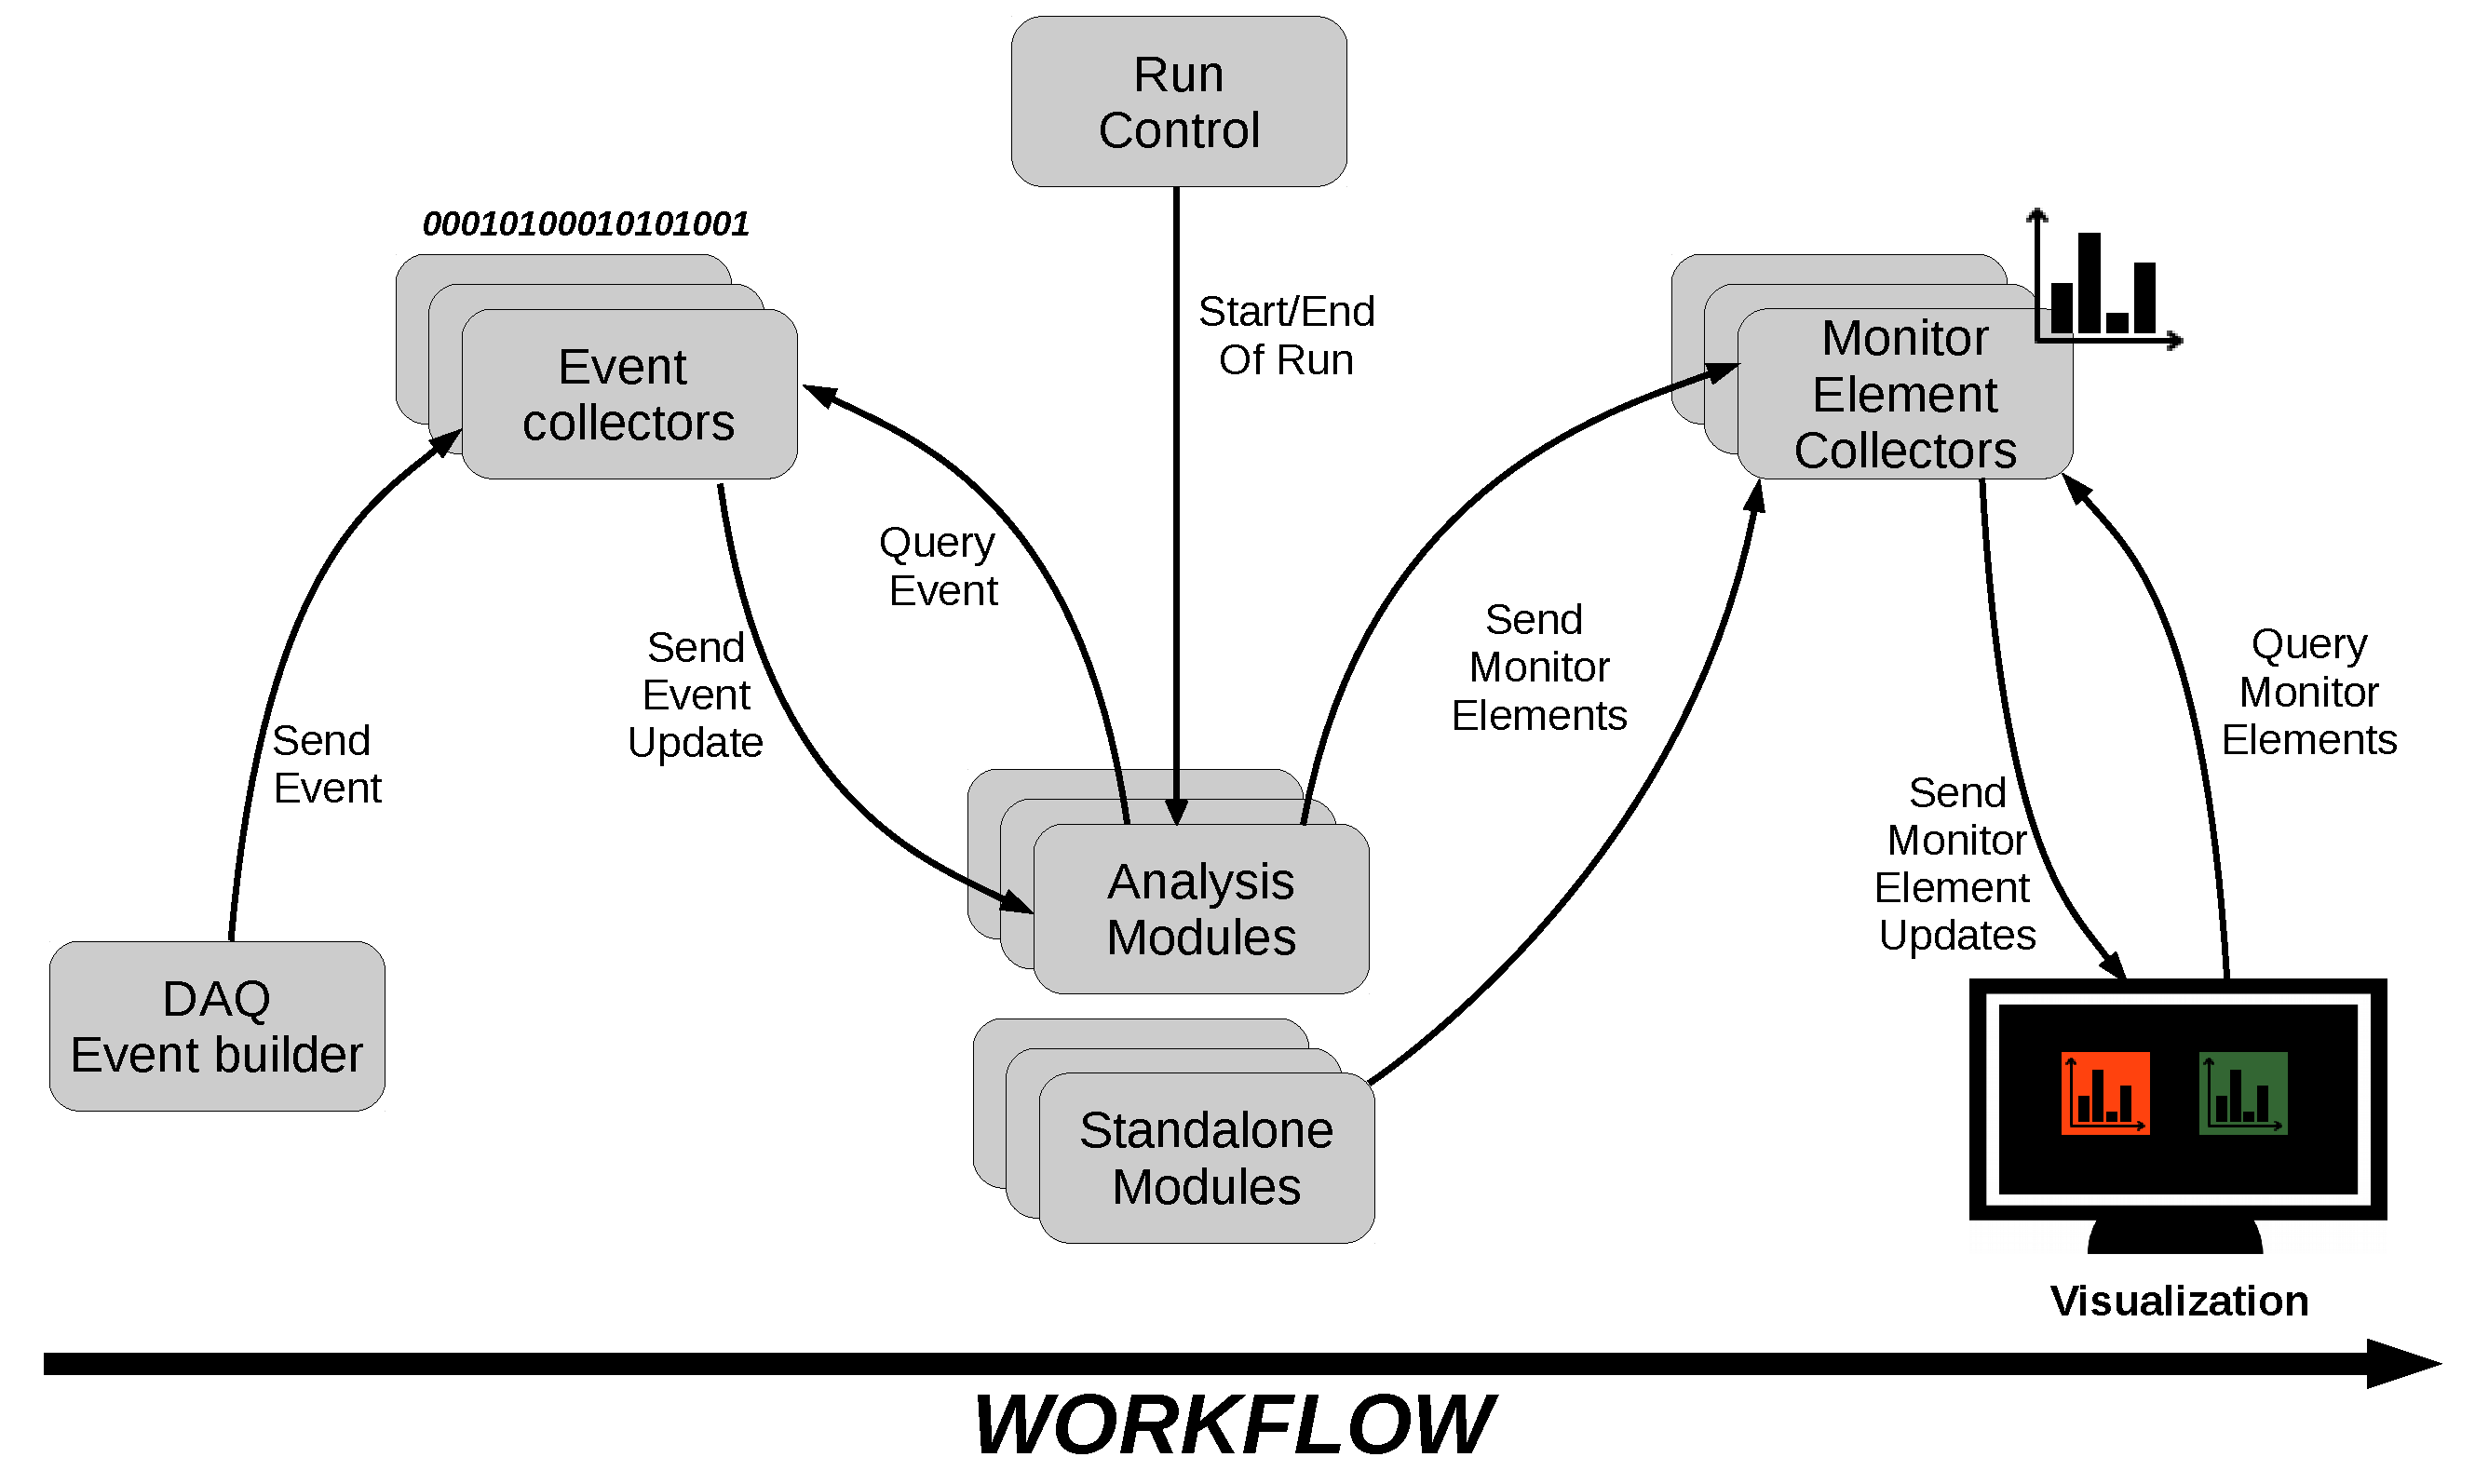
\includegraphics[width=\linewidth]{DQM4HEP_workflow.pdf}
  \end{center}
  \caption{\label{DQM4HEP_WORKFLOW} The DQM data workflow, from the DAQ system to visualization clients}
\end{figure}

First of all, to feed the monitoring system with data, the \verb?levbdim?\footnote{See \href{https://github.com/DQM4HEP/levbdim}{the github page}} software provides functionalities to read data from the shared memory. For the SDHCAL implementation, the DAQ reads data from the shared memory before writing the data to disk. This DAQ process duplicate the data into the shared memory and they are read again by the monitoring system. This process will be labelled as the \textit{\bf shm proxy} afterward in this document.

The monitoring data are then collected by one (or multiple) event collector(s). These server applications are needed to collect the data and make them available to the analysis modules afterward. These processes will be labelled as \textit{\bf event collector}.

Then next step consist in query data and run online analysis. To do that, multiple online analysis are run independently into different processes. These processes will be labelled as \textit{\bf analysis module} afterward. The analyses process events coming from the event collector as soon as the previous event processing is finished and a new event is available. These analysis modules produce histograms, graphs, scalar values, etc ... These elements are labelled as \textit{\bf monitor element}. They encapsulate a ROOT TObject (TH1, TGraph, etc ...) with additional features specific a DQM system such as its quality, quality tests results, etc... To see all the attributes of a monitor element, see the \href{https://github.com/DQM4HEP/DQMCore/blob/master/source/include/dqm4hep/DQMMonitorElement.h}{header file}. These monitor elements are collected by \textit{\bf monitor element collectors} in order to be distributed to shifters on graphical user interfaces. Events are processed during a \textit{\bf cycle}. Different cycle types are available : i) a \textit{\bf timer cycle}, process data during n seconds, ii) an \textit{\bf event counter cycle}, process \textit{n} events. At the end of a cycle, the monitor elements are published into the collector. Note that a \textit{\bf run control} must provide the start of run (\textit{\bf SOR}) and end of run (\textit{\bf EOR}) signals to start and stop the analyses.

The last step in the DQM workflow consists in one or multiple client interfaces to monitor the data taking. On these interfaces, clients can query monitor element to watch and can receive frequent update from the system. Multiple canvas areas are provided to draw multiple monitor elements at the same time. This allows to see correlations when, for instance, problem occurs.
%See the dedicated section (Sec. \ref{DQMVIZ_SECTION}) for more information.


% \begin{wrapfigure}{r}{0.45\textwidth}
%   \vspace{-20pt}
%   \begin{center}
%     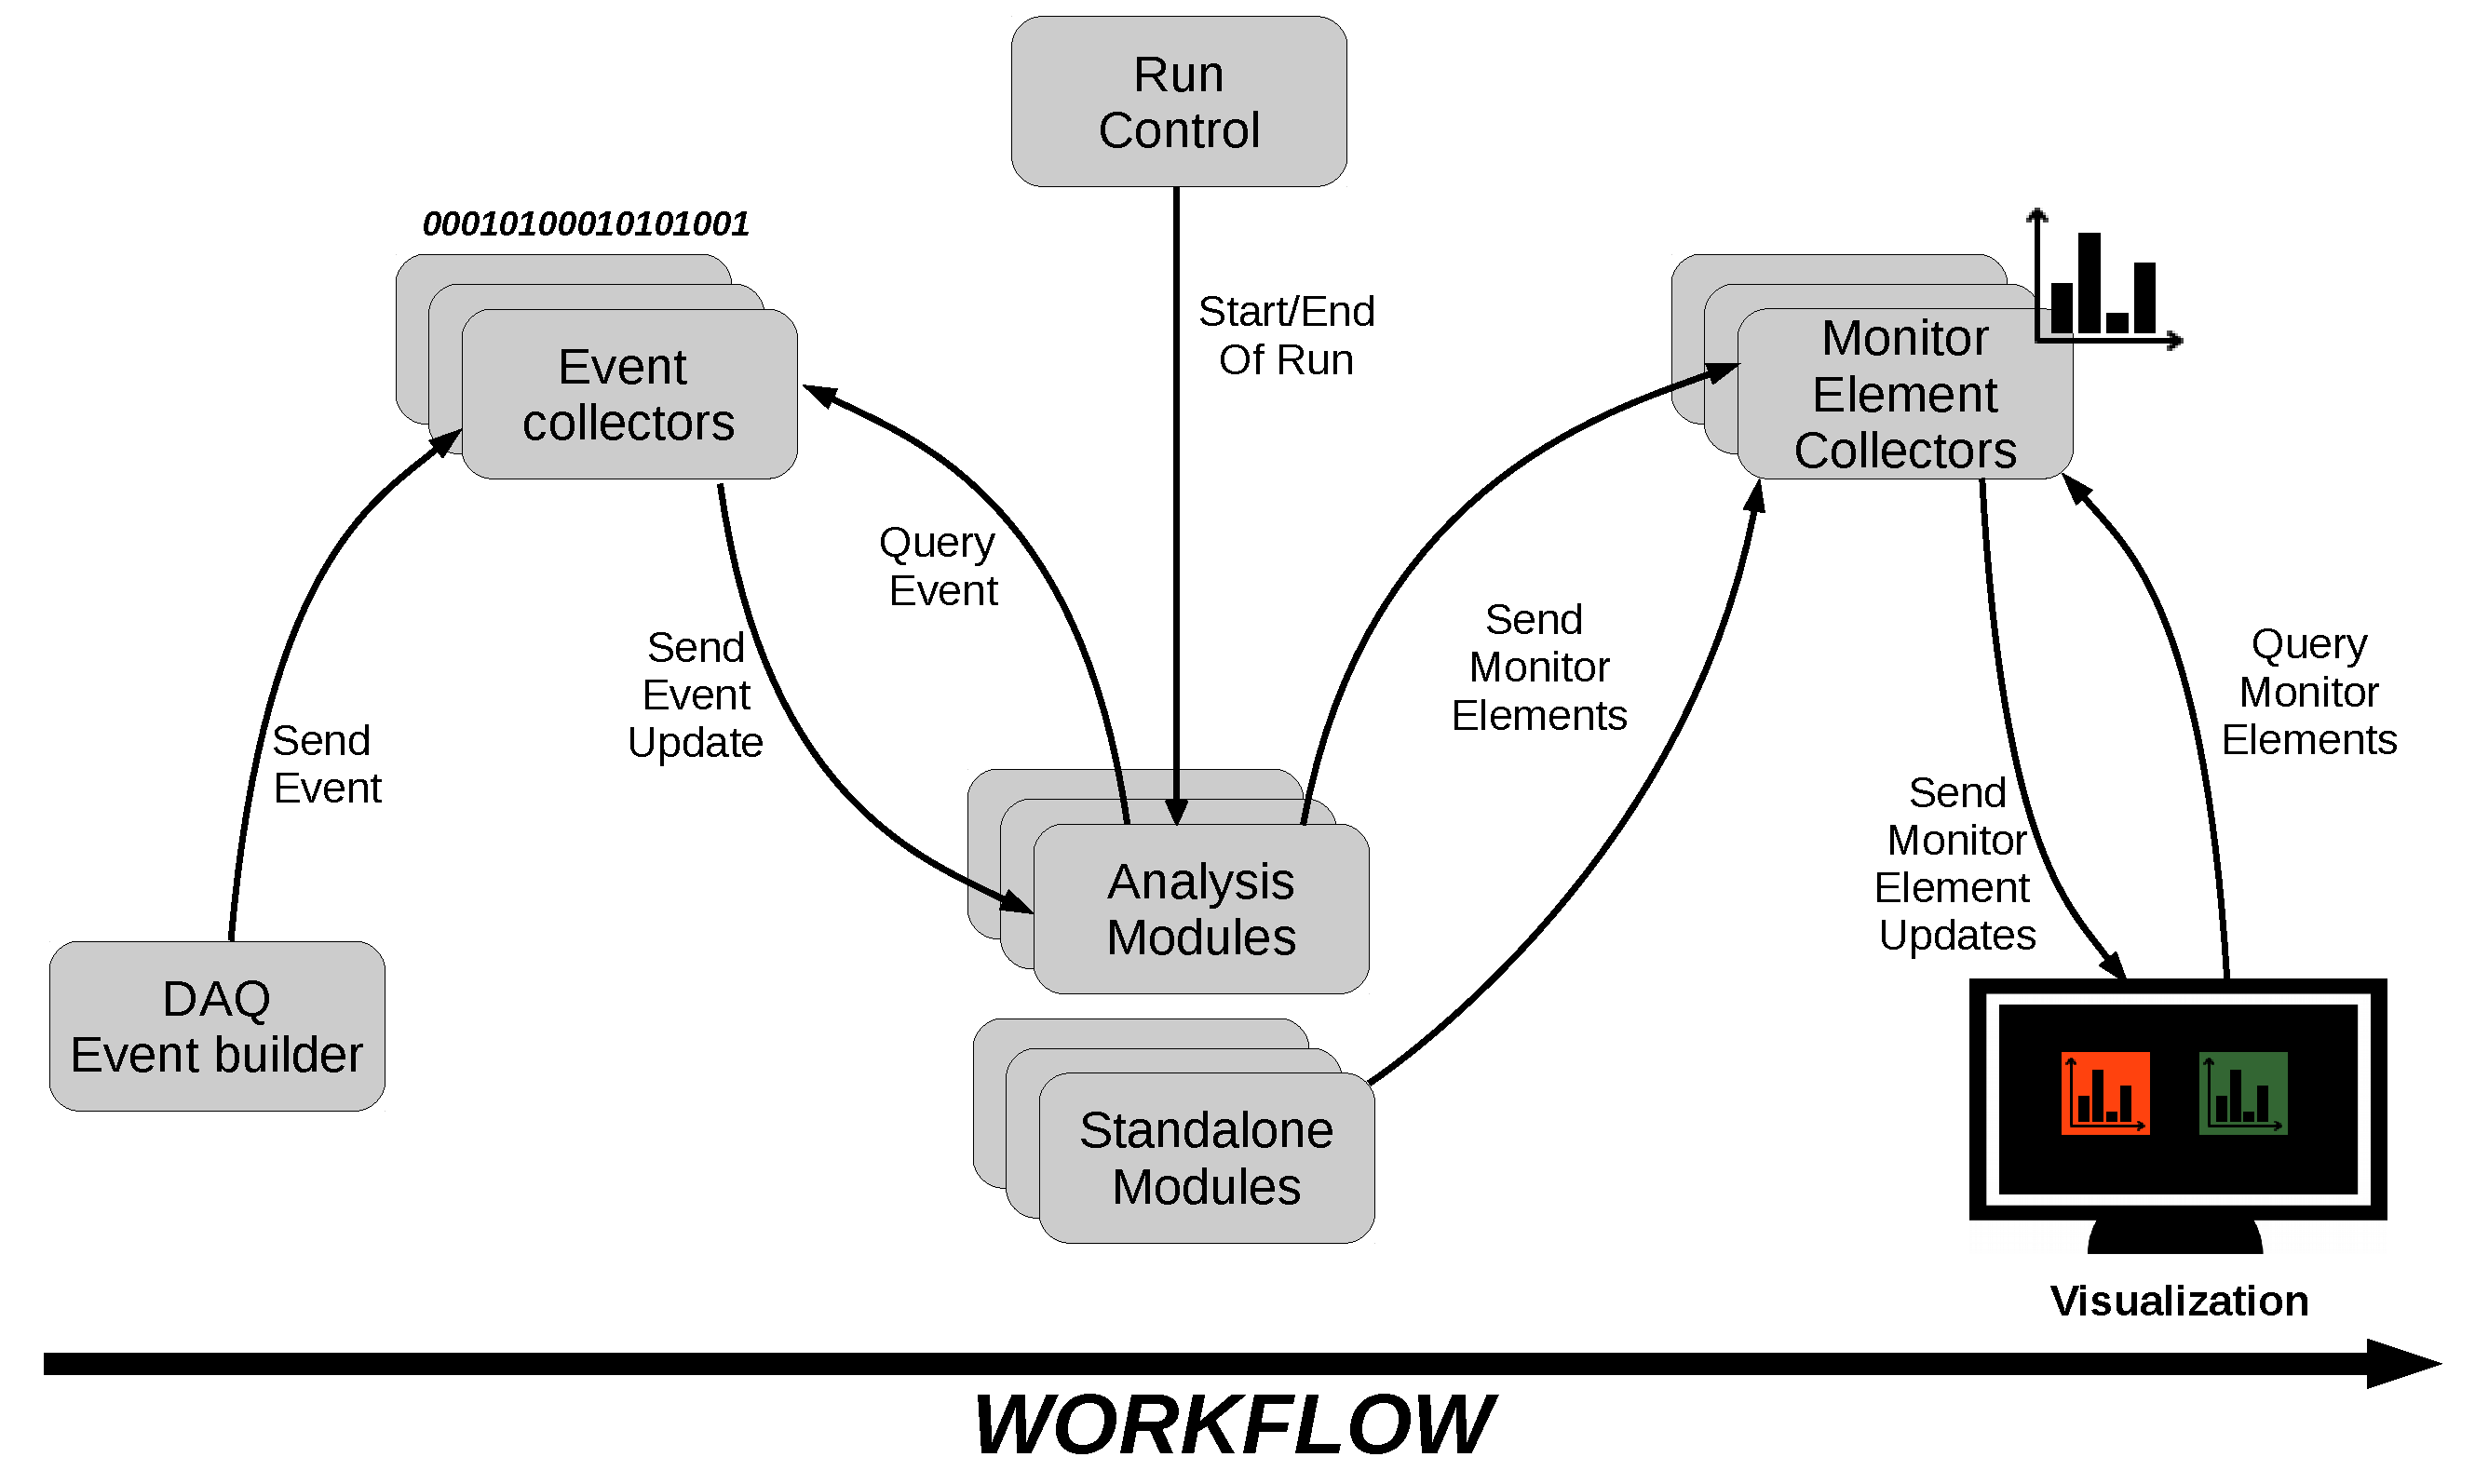
\includegraphics[width=\linewidth]{DQM4HEP_workflow.pdf}
%   \end{center}
%   \vspace{-10pt}
%   \caption{\label{DQM4HEP_WORKFLOW} The DQM data workflow, from the DAQ system to visualization clients}
% \end{wrapfigure}


% \newpage
% \begin{thebibliography}{99}
% 
% \bibitem{ilc-tdr} 
% J. Carwardine {\it et al.},  \emph{International Linear Collider Technical Design Report}. 1) Executive Summary, 2) Physics, 3) Accelerator, 4) Detectors. 12 June 2013
% 
% \bibitem{pandora-pfa}
% M. A. Thomson, \emph{Particle Flow Calorimetry and the PandoraPFA Algorithm}, \href{http://dx.doi.org/10.1016/j.nima.2009.09.009}{\tt 2009, Nucl.Instrum.Meth. A611 25-40}
% 
% \bibitem{calice-pandora-paper}
% The CALICE Collaboration, \emph{Experimental Tests of Particle Flow Calorimetry}, \href{http://www.arxiv.org/abs/1105.3417}{\tt arXiv:1507.05893 [physics.ins-det]}
% 
% \bibitem{sdhcal-paper} 
% The Calice Collaboration, \emph{Construction and commissioning of a technological prototype of a high-granularity semi-digital hadronic calorimeter}. \href{http://dx.doi.org/10.1088/1748-0221/10/10/P10039}{\tt 2015, JINST \textbf{10} P10039}
% 
% \bibitem{arbor-manqi}
% M. Ruan, \emph{Arbor, a new approach of the Particle Flow Algorithm}, Proceeding of CHEF 2013. \href{http://www.arxiv.org/abs/1403.4784}{\tt arXiv:1403.4784 [physics.ins-det]}
% 
% \bibitem{pandora-sdk}
% J. S. Marshall, M. A. Thomson, \emph{The Pandora Software Development Kit for Pattern Recognition}, \href{http://dx.doi.org/10.1140/epjc/s10052-015-3659-3}{\tt 2015, Eur.Phys.J. C75 439}
% 
% \bibitem{marlin-lccd}
% F. Gaede, {\it Marlin and LCCD: Software tools for the ILC}, \href{http://dx.doi.org/10.1016/j.nima.2005.11.138}{\tt Nucl.Instrum.Meth. A559 (2006) 177-180}
% 
% \bibitem{ilcsoft}
% ILCsoft, 2012. \href{http://ilcsoft.desy.de/portal}{\tt http://ilcsoft.desy.de/portal}
% 
% \bibitem{hadron-jets} 
% O. Lobban, A. Sriharan, R. Wigmans,  \emph{On the energy measurement of hadron jets}, \href{http://dx.doi.org/10.1016/S0168-9002(02)01615-7}{\tt Nucl.Instrum.Meth. A495 (2002) 107-120}
% 
% \end{thebibliography}
% 

\end{document}
